\subsection{Government and Licensing}
\label{subsec:intro:gov lic}

In \CVCV, Government and Licensing are opposing forces:
While Government inhibits the melodic expression of
its target, Licensing makes it stronger.

Where in \cite{scheer2004} both forces are independent
from each other (a constituent can be both governed
and licensed, in which case both forces cancel out),
\cite{scheer2012} refines the model as follows:
\blockquote[\cite{scheer2012}]{
  (68) government over licensing
  
  no constituent can be governed and licensed at the
  same time. In case a constituent can potentially be
  subject to both lateral forces, it will be governed.
}
\TODO{is this relevant to German? maybe just mention but ignore it afterwards}

Each Nucleus always \wordunsure{exhibits}
all available forces: full vowels govern and license
while the ability of schwa and final empty Nuclei to
govern/license is subject to (separate) language-specific
parametrization.
In german, both schwa and final empty Nuclei govern but
do not license.

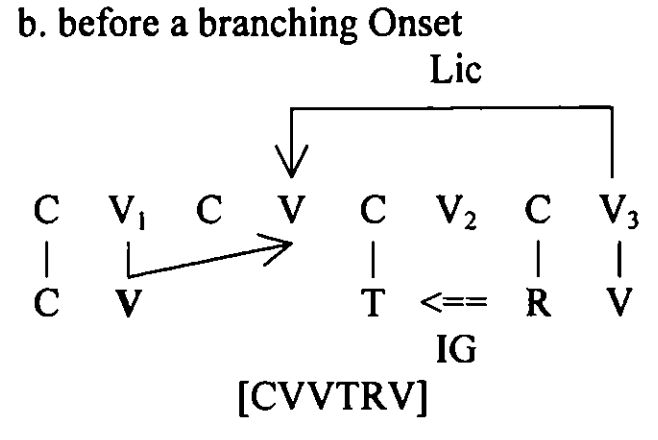
\includegraphics[width=.5\textwidth]{figures/lic-over-branching-onset.png}

\textquote[{\cite[p.~144]{scheer2012}}]{
  Government and licensing must be counted out because they represent
  phonological computation, rather than representational objects,
  and hence cannot be stored in the lexicon (see §186).
}

\subsection[TODO]{\TODO{}}
\begin{itemize}\color{red}
  \item Domains
  \item \gls{FEN}
  \item concept: relations have a head
  \item long vowels: complement needs to be licensed
  \item \gls{ECP}
  \item FEN cannot govern alternation sites:\\
    \textquote[{\cite[p.~643]{scheer2004}}]{%
      Final empty Nuclei can only govern Nuclei that are bare
      of any underlying melody (floating or attached)}
\end{itemize}